\chapter{Modelo Computacional} \label{metodologia:modelocomputacional}

Usando todas las curvas de luz disponible para el sistema \atoObjId se puede
generar un modelo computacional cuyos parámetros físicos resultan en una curva
de luz sintética que explique de manera adecuada las curvas fotométricas
observadas. Este método al final daría como resultado una \textit{solución
fotométrica} del sistema, en el cual se reportan los valores óptimos de cada
parámetro y la incertidumbre dada por la calidad de los datos. A continuación se
plasma el proceso que se llevó a cabo para llegar a una solución fotométrica del
sistema \atoObjIdNoSpace; debido a la alta dimensionalidad del problema de
sistemas binarios estelares, no se puede garantizar que esta sea la única
combinación de parámetros que mejor ajusten el modelo a los datos, aunque esta
posibilidad es mitigada utilizando las herramientas disponibles en PHOEBE.

\section{Preparación del Modelo}

El modelo en PHOEBE (llamado \textit{bundle} en inglés por el nombre de la clase
\code{phoebe.Bundle}) necesita ser preparado al principio para empezar el
proceso de ajuste. Esto incluye cargar las curvas fotométricas observadas de
cada catálogo al bundle; PHOEBE requiere que estas sean en arreglos de tiempo,
flujos, y errores de flujo\textemdash las mediciones de flujo se deben a que
PHOEBE no trabaja de manera directa con magnitudes, y los errores son necesarios
para que las herramientas de optimización de parámetros puedan funcionar
adecuadamente. En el Notebook
\href{https://github.com/KnightIV/UANL_MAPTA_Observaciones/blob/main/analisis/phoebe_model/initial-model-prep.ipynb}{\code{initial-model-prep.ipynb}}
está el código que se utilizó para cargar los datos de Iturbide, Gaia, y ZTF al
bundle en el que se trabajó; esto incluye realizar una limpieza de las curvas de
luz. Esto es más evidente en las curvas de luz en fase vistas en la
\reffigure{figuraGaiaIturbideZtfCurvasFase} donde se aprecia que varias
observaciones quedan fuera de la forma general aparente de su curva de luz
respectiva. Las observaciones más erróneas se pueden eliminar utilizando las
banderas (\textit{flags} como se identifican en los datos) que marcan los
problemas que sucedieron durante las observaciones. Para los pocos puntos que
quedaron fuera del rango de la curva de luz promedio se utilizaron límites de
flujo manuales en base a las gráficas vistas en la
\reffigure{figuraGaiaIturbideZtfCurvasFase}. Cada punto contribuye al cálculo de
la función de costo que parametriza la calidad del ajuste, por lo cual es
importante eliminar aquellos datos que tendrían un efecto negativo
significativo, afectando algoritmos que buscan optimizar el valor de esta
función.

Una optimización empleada en el cómputo del modelo hacia adelante es limitar los
puntos de tiempo para el cual se calcula el flujo recibido del sistema. Esto es
necesario para limitar el tiempo de ejecución del programa, en particular para
los procesos de optimización y muestreo MCMC que corren por varias iteraciones,
calculando el modelo sintético en cada iteración. PHOEBE utiliza los valores de
los tiempos de las curvas de luz proporcionadas para calcular el modelo hacia
adelante, lo cual causa que el modelo tarde varios minutos para generar la curva
sintética. Para declarar las fases de cómputo de manera explicita se utiliza el
siguiente código (implementado en el Notebook
\href{https://github.com/KnightIV/UANL_MAPTA_PlanObservaciones/blob/main/analisis/phoebe_model/estimations/ebai-default.ipynb}{\code{ebai-default.ipynb}}),
visto en la \refcode{codigoOptimizandoFasesComputoPhoebe}. El cálculo del modelo
hacia adelante en PHOEBE es en función de tiempo, no de fase, por lo cual PHOEBE
genera una lista de tiempos para el cual computar el modelo utilizando la
función \code{phases\_to\_times}, tomando como argumentos el periodo del
sistema, el tiempo de conjunción superior, y el cambio del periodo orbital con
el tiempo ($\mathrm{d}P_{\mathrm{orb}} / \mathrm{d}t$) en el caso de ser
distinto a 0. Los tiempos generados por esta función no se transforman a los
tiempos de las observaciones, pero debido a que el modelo sintético es evaluado
únicamente en fase esto no es un requisito importante para este estudio. El
tiempo de cómputo para el modelo hacia adelante de las curvas de ZTF:g y ZTF:r
se redujo de 10 minutos por modelo a aproximadamente 1 minuto por modelo.

\begin{figure}[!ht]
    \begin{lstlisting}[language=Python, autogobble]
        import phoebe

        # b: phoebe.Bundle
        b.flip_constraint('compute_phases@lcZtfG', 
            solve_for='compute_times@lcZtfG')
        b.set_value(qualifier='compute_phases', 
            dataset='lcZtfG', 
            value=phoebe.linspace(-0.5, 0.5, num=151, endpoint=True))
    \end{lstlisting}
    \caption{Estableciendo valores fijos de las fases orbitales para cuales
    calcular el modelo hacia adelante para la curva de luz \code{lcZtfG} en la
    pasabanda ZTF:g. La función \code{phoebe.linspace} genera una lista de
    valores numéricos en el intervalo $[-0.5, 0.5]$ de 151 elementos, una
    disminución significativa de los 453 puntos de tiempo en la curva observada
    de ZTF:g.}
    \label{codigoOptimizandoFasesComputoPhoebe}
\end{figure}

\section{Estimaciones Iniciales}

Una vez determinado el periodo orbital del sistema se puede empezar un estudio
de la morfología de las curvas de luz en fase, cuya forma se relaciona
directamente con parámetros físicos del sistema. PHOEBE ofrece distintos métodos
para generar las primeras estimaciones de los parámetros del sistema. El
estimador \textbf{EBAI-KNN} (descrito en la
\refthesissubsubsection{intro:phoebe:problema_inverso:ebai}) es capaz de estimar
los siguientes parámetros: el \textit{tiempo de conjunción superior}
(\code{t0\_supconj}), la \textit{razón de temperaturas} (\code{teffratio}), la
\textit{inclinación orbital} (\code{incl@binary}), el \textit{factor de relleno}
(\textit{fillout factor} en inglés, \code{fillout\_factor}), y la \textit{razón
de masas} (\code{q}). A pesar que dentro de PHOEBE estén implementados
estimadores adicionales, solo se puede aplicar el \textbf{EBAI-KNN} estimador;
esto se debe a que el modelo del sistema del que parte este trabajo corresponde
al de una binaria en contacto (elegido por la morfología aparente de la curva de
luz de Iturbide). Para poder adoptar los valores propuestos por los estimadores
fue necesario eliminar el constreñimiento puesto por PHOEBE en el parámetro
\code{fillout\_factor}. Este parámetro está constreñido por la función interna
de PHOEBE \code{pot\_to\_fillout\_factor}, la cual toma como entrada la razón de
masa \code{q} y el valor del potencial de Roche $\Omega$ que coincide con la
superficie delimitada por la envoltura común de una binaria en contacto. Como
resultado el parámetro \code{fillout\_factor} queda constreñido por los
parámetros \code{pot@contact\_envelope} y el radio de la estrella primaria
\code{requiv}, lo que efectivamente significa que los radios del sistema binario
quedan parametrizados por el factor de relleno. 

Dentro del Jupyter Notebook
\href{https://github.com/KnightIV/UANL_MAPTA_PlanObservaciones/blob/main/analisis/phoebe_model/estimations/ebai-default.ipynb}{\code{ebai-default.ipynb}}
se puede encontrar el código con el que se llevaron a cabo las pruebas de
estimación de parámetros. El estimador \textbf{EBAI-KNN} puede que obtenga
diferentes soluciones del sistema dependiendo de la curva de luz utilizada; por
lo cual se esperaba que obtuviera diferentes resultados dependiendo de las curvas
de entrada. Para obtener un panorama completo de las posibles soluciones
fotométricas so ejecutaron varios estimadores de PHOEBE, cada uno operando sobre
una diferente combinación de curvas de luz; se corrió un estimador por cada
curva de luz individual, al igual que unos estimadores que tuvieron de entrada
una combinación de curvas de luz de Gaia, Iturbide, y ZTF, con la finalidad de
experimentar con las capacidades de PHOEBE. El experimento completo junto a sus
curvas de luz sintéticas correspondientes se pueden ver en el Notebook
antedicho, acompañado de las gráficas resultantes de cada estimador.

\subsection{Elección del Modelo Inicial}

Una consideración importante en el proceso de modelación computacional es la
existencia de diferentes soluciones fotométricas dado un mismo conjunto de
datos. Esto se debe a la ortogonalidad de los parámetros en el sistema; dos o
más parámetros pueden estar correlacionados el uno al otro, lo cual significa
que no existe una solución única correcta del sistema. Para decidir entre los
varios estimadores se tomó como criterio de selección el ajuste del modelo hacia
adelante utilizando la métrica definida en la
\refequation{ecuacionLambdaCostoPhoebe}, $\lambda$, la cual está normalizada al
número de puntos en las curvas de luz observadas. Estos se pueden ver en la
\reffigure{figuraEstimadoresLambda}. Viendo solo la medida del ajuste $\lambda$
total para cada modelo se llegaría a la conclusión que el modelo
\code{ebai\_knn\_ztf\_solution} es el que más coincide con los datos
observacionales. Sin embargo, es necesario no solo ver el ajuste a cada curva de
luz individual, pero también considerar los valores físicos obtenidos del
estimador. Un criterio que empleamos fue adoptar la solución cuya razón de masa
\code{q} sea la más cercana al valor obtenido utilizando la red neuronal
desarrollada por
\citeyearparen{poro_investigation_of_orbital_period_mass_relations_2022}. Dado
el periodo orbital de $8.01 \ \mathrm{d}$ obtenemos un valor estimado de
aproximadamente $0.692$; de este se obtiene $1/q \approx 1.444$, el cual es
importante tener en mente ya que \code{q} en PHOEBE no está restringido al
intervalo $(0, 1]$ como en el modelo de
\citeyearparen{poro_investigation_of_orbital_period_mass_relations_2022}. Por lo
tanto se eligió las estimaciones de \code{ebai\_knn\_ztf\_gaia\_solution}, el
cual utilizó la fotometría de Gaia y ZTF.El resultado inicial del modelo se
puede ver en la \reffigure{figuraEstimacionInicialModelo}, junto a los
parámetros del modelo en la \reftable{ebaiKnnInitialEstimationsValues}.

\begin{figure}[!ht]
	\centering
	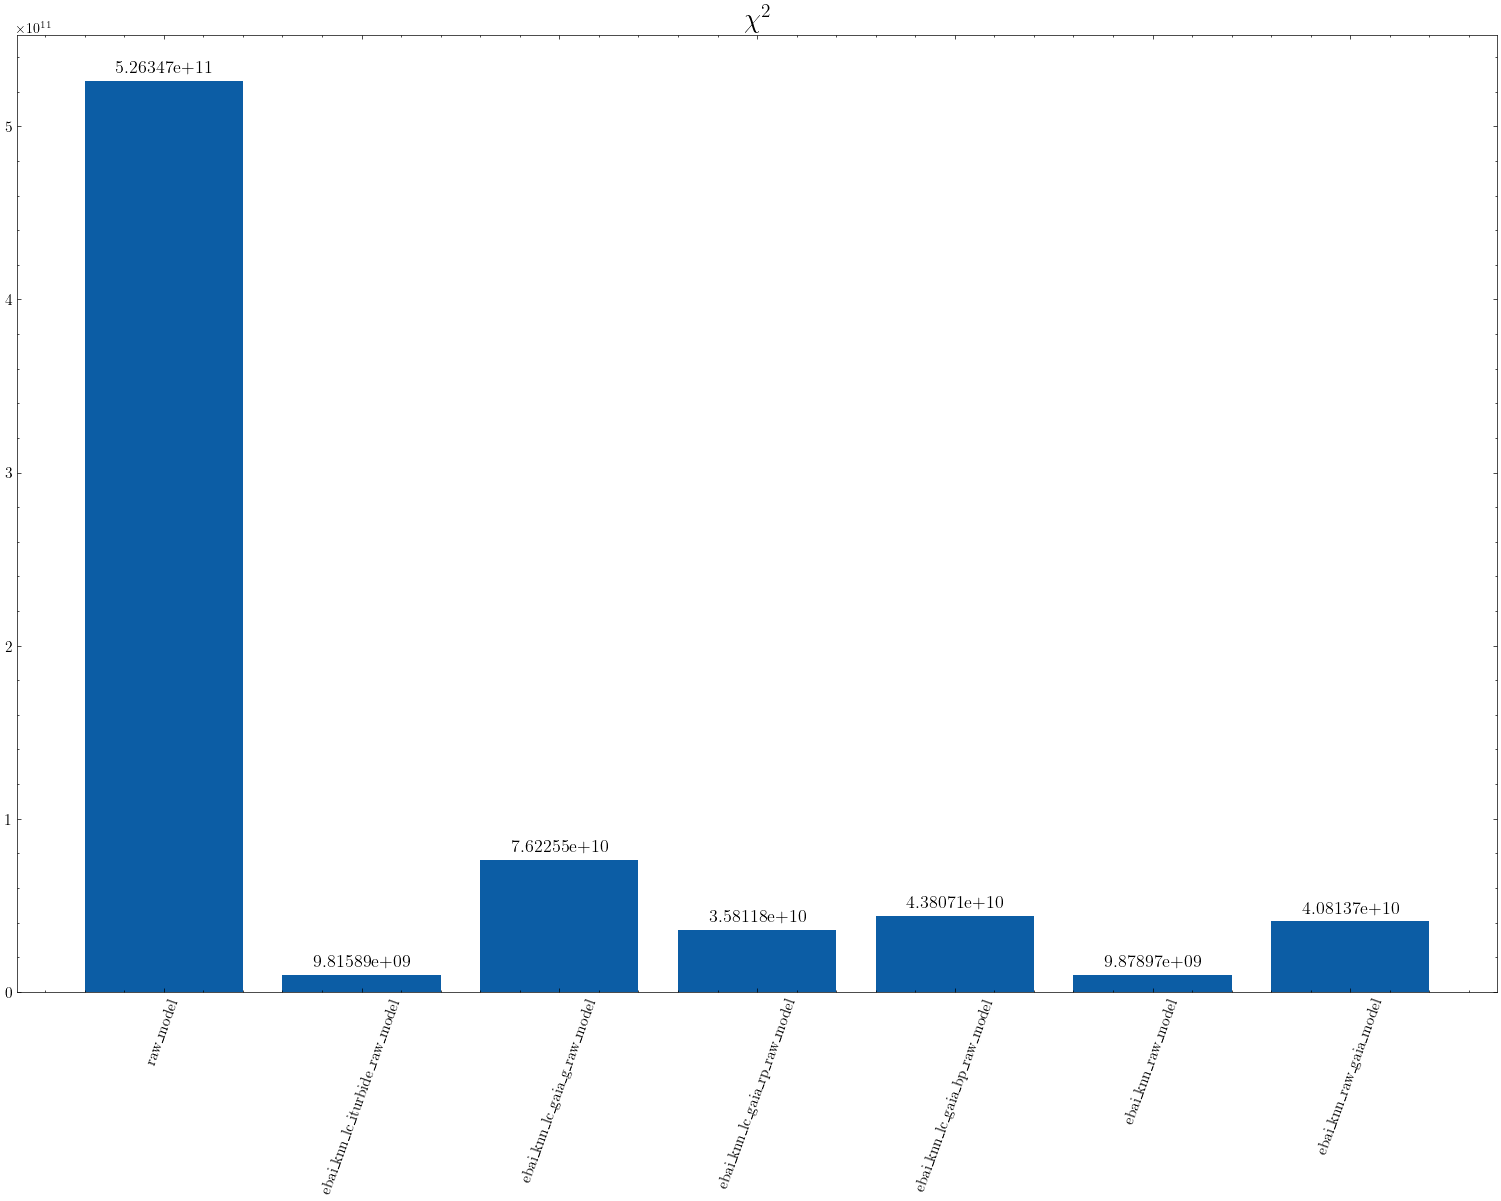
\includegraphics[scale=0.6]{Metodologia/Secciones/ModeloComputacional/Figures/EstimadoresChiResultados.png}

	\caption{Resultados del ajuste ($\lambda$) de los modelos sintéticos
		generados utilizando los parámetros dados por cada estimador. Cada
		estadística fue calculada con respecto a todos los datos observacionales
		disponibles, sin importar las combinaciones de curvas de luz utilizadas
		para hacer la estimación. \code{default\_model} corresponde al modelo
		inicial que ofrece PHOEBE a través de la función
		\code{phoebe.default\_contact\_binary()}. Los nombres de los estimadores
		en el eje vertical de la gráfica indican los datos observacionales
		utilizados para cada estimación de parámetros, junto al valor del ajuste
		el modelo sintético a todas las curvas del modelo. }
	\label{figuraEstimadoresLambda}
\end{figure}

\begin{figure}[!ht]
	\centering
	\xincludegraphics[scale=0.41]{Metodologia/Secciones/ModeloComputacional/Figures/ebaiKnnIturbideNorm.png}
	\xincludegraphics[scale=0.41]{Metodologia/Secciones/ModeloComputacional/Figures/ebaiKnnGaiaRaw.png}
	\xincludegraphics[scale=0.41]{Metodologia/Secciones/ModeloComputacional/Figures/ebaiKnnZtf.png}

	\caption{Modelos sintéticos del modelo utilizando los parámetros estimados
	por \code{ebai\_knn\_ztf\_gaia\_solver} junto a los residuos en los flujos
	para cada curva de luz. Estos modelos fueron sintetizados utilizando un
	factor de escala de flujos flexible, utilizando la opción \code{pblum\_mode
	= "dataset\_scaled"}, el cual nos permite analizar la morfología del modelo
	sintético sin considerar por ahora el efecto en la escala de la curva de
	parámetros relacionados con la luminosidad de cada componente, como las
	temperaturas absolutas o los radios de ambas estrellas. Estos parámetros son
	ajustados en los siguientes pasos de afinación del modelo.}
	\label{figuraEstimacionInicialModelo}
\end{figure}

% TODO: style table
\begin{table}[!ht]
	\centering
	\begin{tabular}{|l|l|}
		\hline
		% \rowcolor{blue}
		\thead{Parámetro}                        & \thead{Valor} \\
		\hline
		\code{t0\_supconj@binary}                & 0.02571 d    \\
		\hline
		\code{teffratio@binary}                  & 0.98746       \\
		\hline
		\code{incl@binary}                       & 70.3197 deg  \\
		\hline
		\code{fillout\_factor@contact\_envelope} & 0.25767       \\
		\hline
		\code{q@binary}                          & 1.93380       \\
		\hline
	\end{tabular}
	\caption{Resultados adoptados de las estimaciones iniciales, utilizando el
		estimador cuyos datos de entrada fueron las curvas de Gaia y ZTF. Las
		unidades de cada valor son especificadas excepto para los parámetros
		adimensionales.}
	\label{ebaiKnnInitialEstimationsValues}
\end{table}

\section{Optimización de Parámetros}

Como se puede ver en la \reffigure{figuraEstimacionInicialModelo} el modelo
inicial de PHOEBE no se ajusta perfectamente bien a los dados datos
observacionales, visto en los residuos de cada curva de luz. En la siguiente
etapa del proyecto se emplea un muestreo MCMC, el cual en teoría es capaz de
determinar el mínimo global del espacio de parámetros, pero a un costo
computacional que crece exponencialmente con la distancia de los parámetros del
sistema actuales al mínimo global de la función de calidad.

El proceso de optimización de parámetros es distinto para cada sistema modelado;
ciertas estrategias pueden funcionar para un sistema y al mismo tiempo no llegar
a una solución adecuada para otro sistema con distintos datos. Para el ajuste de
\atoObjId primero se ajustó el tiempo de superconjunción; esto es visto en los
eclipses del modelo sintético desfasado con los eclipses de las curvas
observadas en la \reffigure{figuraEstimacionInicialModelo}. Esto resultó en un
nuevo valor de $0.02589 \ \mathrm{d}$. Utilizando un optimizador de Nelder Mead
Simplex (\textit{NMS}, descrito en la
\refthesissubsubsection{intro:phoebe:nelder_mead}) se buscó optimizar los mismos
parámetros configurados en la estimación inicial del modelo. Con la finalidad de
obtener un ajuste consistente y solo utilizar datos de alta calidad solo se
utilizó las dos curvas de luz de ZTF para el resto del ajuste del modelo. Esto
se debe al número de buenas observaciones en estos datos; son más numerosas de
las observaciones hechas por Gaia, y son de mejor calidad que las realizadas
desde el OAU. Al tener observaciones simultaneas en diferentes pasabandas
también es posible determinar las temperaturas efectivas de las componentes
estelares. 

El primer optimizador NMS corrigió la razón de temperaturas efectivas
\code{teffratio} (el cual sirve para modificar la luminosidad relativa de la
estrella secundaria con respecto a la primaria, ajustando la profundidad del
eclipse secundario con respecto al eclipse primario), el factor de relleno
\code{fillout\_factor} (que sirve como una parametrización de la razón de radios
de las estrellas, ajustando el ancho de ambos eclipses), la inclinación orbital
del sistema \code{incl@binary} (que dicta el aspecto de los eclipses observados
con respecto al plano de observación, determinando la profundidad y la agudeza
de los eclipses), y la razón de masa \code{q}. La razón de masa no es un
parámetro que se pueda constreñir bien utilizando solo información fotométrica;
esto se debe a las correlaciones presentes en el modelo con los demás parámetros
del sistema. Después de 114 iteraciones el optimizador logró converger a una
solución dada en la \reftable{tablaOptNmResultados}.

% TODO: style table
\begin{table}[!ht]
	\centering
	\begin{tabular}{|l|l|}
		\hline
		% \rowcolor{blue}
		\thead{Parámetro}                        & \thead{Valor optimizado} \\
		\hline
		\code{teffratio@binary}                  & 1.07991       \\
		\hline
		\code{incl@binary}                       & 70.19810 deg  \\
		\hline
		\code{fillout\_factor@contact\_envelope} & 0.09356       \\
		\hline
		\code{q@binary}                          & 2.13478       \\
		\hline
	\end{tabular}
	\caption{Valores optimizados utilizando el algoritmo Nelder-Mead Simplex.}
	\label{tablaOptNmResultados}
\end{table}

\begin{figure}
	\centering
	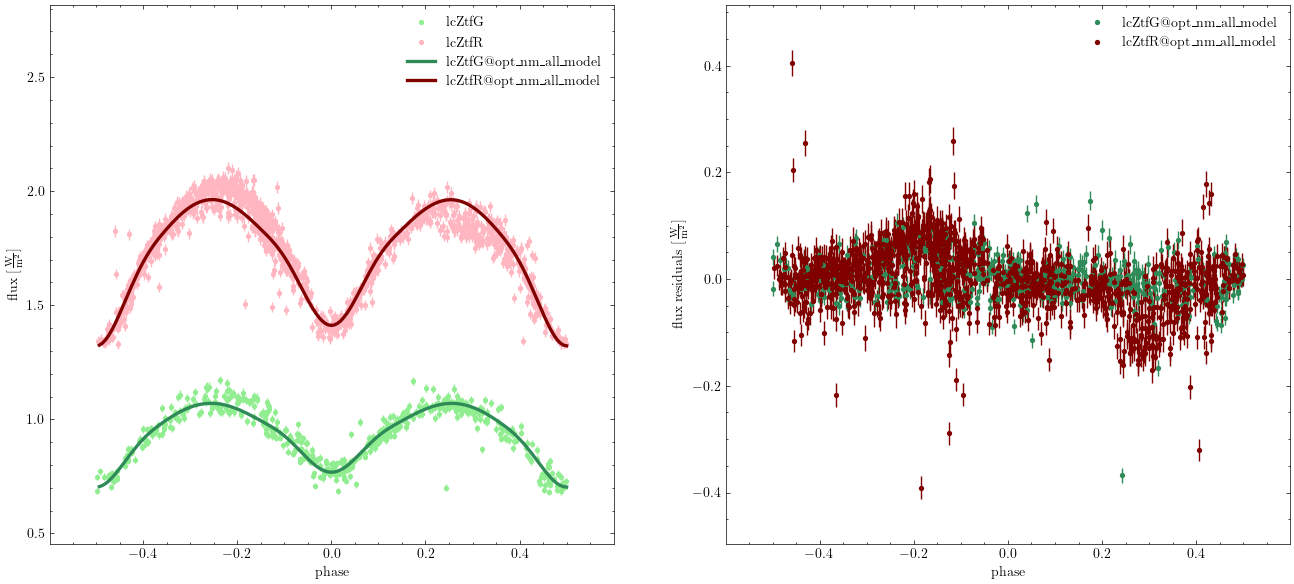
\includegraphics[scale=0.5]{Metodologia/Secciones/ModeloComputacional/Figures/Figura Opt NM Resultados ZTF.png}
	\caption{Modelo sintético generado utilizando los parámetros dados por el
	optimizador NMS, vistos en la \reftable{tablaOptNmResultados}, utilizando el
	tiempo de superconjunción corregido.}
	\label{figuraOptNmResultadosZtf}
\end{figure}

La curva sintética del modelo optimizado visto en la
\reffigure{figuraOptNmResultadosZtf} muestra una asimetría en las jorobas de la
curva de luz en fase. Estos máximos corresponden a las fases orbitales en las
cuales la mayor cantidad de elementos superficiales de ambas componentes
coinciden con nuestra línea de observación. Este fenómeno se le denomina el
\textit{efecto O'Connell}, descrito originalmente por
\citeyearparen{oconnell_periastron_effect-OConnell_effect_1951} donde se
distingue del efecto de periastro que es causado por efectos de marea en
sistemas con órbitas excéntricas. El \textit{efecto O'Connell} se debe a la
diferencia de luminosidad entre diferentes hemisferios de una estrella; puede
ser causado por un punto caliente debido a la acreción de material en el caso de
haber una alta tasa de transferencia de masa
[\citeyearparen{darwish_light_curve_analysis_four_new_short_period_eclipsing_binaries_2024}],
o por manchas en la superficie estelar debido a actividad en la fotósfera. Para
llegar a un mejor ajuste de la curva fotométrica se introdujo una mancha fría en
la estrella secundaria. Después de hacer un ajuste manual de los parámetros de
la mancha se utilizó un optimizador NMS para obtener los parámetros óptimos de
la mancha estelar. Los parámetros optimizados se pueden ver en la
\reftable{tablaOptManchaResultados}, y la mancha estelar se puede ver
representada en la \reffigure{figuraMallaManchaNm}.

% TODO: style table
\begin{table}[!ht]
	\centering
	\begin{tabular}{|l|l|}
		\hline
		% \rowcolor{blue}
		\thead{Parámetro}	& \thead{Valor optimizado} \\
		\hline
		\code{colat}	& 89.77983 deg	\\
		\hline
		\code{long}		& 81.09966 deg  \\
		\hline
		\code{radius} 	& 25.12086 deg	\\
		\hline
		\code{relteff}	& 0.93007		\\
		\hline
	\end{tabular}
	\caption{Parámetros de la mancha estelar optimizados utilizando el algoritmo
	Nelder-Mead Simplex, el cual logró converger después de 102 iteraciones.
	Todos los parámetros son relativos a la superficie estelar a la que le
	pertenece la mancha; la longitud \code{long} donde se define la longitud
	$0^{\circ}$ viendo a la estrella primaria, la latitud \code{colat} se define
	como el ángulo polar empezando desde el polo norte de la estrella, el radio
	angular \code{radius}, y la temperatura efectiva relativa \code{relteff} con
	respecto a la temperatura superficial.}
	\label{tablaOptManchaResultados}
\end{table}

\begin{figure}[!ht]
	\centering
	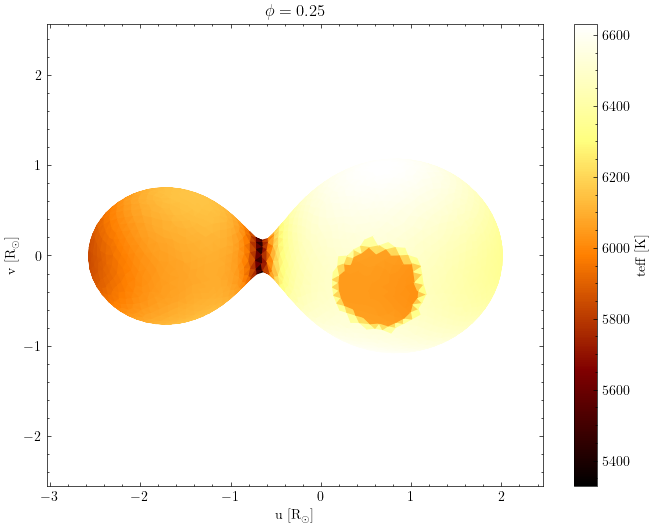
\includegraphics[scale=0.8]{Metodologia/Secciones/ModeloComputacional/Figures/Figura Malla Mancha NM.png}
	\caption{Malla representando la superficie estelar de ambas componentes en
	su fase orbital $\phi = 0.25$, en el máximo menor de la curva fotométrica.
	Aquí se puede apreciar la mancha estelar introducida a la componente
	secundaria. La temperatura efectiva de cada elemento superficial de la
	envoltura en común, donde la mancha se ve de un color más oscuro debido a su
	baja temperatura con respecto al resto de la superficie estelar.}
	\label{figuraMallaManchaNm}
\end{figure}

Una vez que se haya llegado a un nivel de ajuste adecuado con los optimizadores
de tipo NMS se aplicó un último ajuste utilizando correcciones diferenciales,
los cuales funcionan mejor cuando los parámetros se encuentren lo
suficientemente cerca del mínimo global, para evitar caer y estar atrapados
dentro de un mínimo local. El motivo para acercarnos lo más posible al mínimo
global es para reducir el trabajo del muestreo MCMC; entre mayor sea la
distancia que los caminadores tengan que recorrer, se requerirá más iteraciones
para obtener un muestreo adecuado del espacio de parámetros. El resolvedor se
crea con el código en la \refcode{codigoOptimizadorDc}, en donde se define el
tamaño de los pasos que intenta hacer el optimizador; estos deben de ser
suficientemente pequeños para evitar saltos fuera del área de interés, pero
suficientemente grandes para que haya un cambio en el ajuste del modelo. El
tamaño de los pasos se determinó por medio de experimentación manual del efecto
en un modelo sintético de PHOEBE.

\begin{figure}[!ht]
	\begin{lstlisting}[language=Python, autogobble]
		b.add_solver('optimizer.differential_corrections', solver='dc_relative', overwrite=True,
             fit_parameters=['teffratio', 'incl@binary', 'fillout_factor', 'q'],
             steps={
                'q': 0.01,
                'incl@binary': 1,
                'fillout_factor': 0.01,
                'teffratio': 0.01
             })
	\end{lstlisting}
	\caption{Código que se utilizó para crear el optimizador de correcciones
	diferenciales para los parámetros que dictan la forma de la curva de luz en
	fase. El argumento \code{steps} del optimizador representa $\Delta
	\mathbf{p} = \{ \Delta p_1, ..., \Delta p_k \}$ visto en la
	\refequation{ecuacionDiferenciasFinitas}.}
	\label{codigoOptimizadorDc}
\end{figure}

% TODO: style table
\begin{table}[!ht]
	\centering
	\begin{tabular}{|l|l|}
		\hline
		% \rowcolor{blue}
		\thead{Parámetro}                        & \thead{Valor optimizado} \\
		\hline
		\code{teffratio@binary}                  & 1.06676       \\
		\hline
		\code{incl@binary}                       & 68.42157 deg  \\
		\hline
		\code{fillout\_factor@contact\_envelope} & 0.07892       \\
		\hline
		\code{q@binary}                          & 1.10457       \\
		\hline
	\end{tabular}
	\caption{Valores optimizados utilizando un optimizador de correcciones diferenciales.}
	\label{tablaOptDcResultados}
\end{table}

Después de 17 iteración se obtuvieron los parámetros vistos en la
\reftable{tablaOptDcResultados}, de los cuales se generó las curvas sintéticas
vistas en la \reffigure{figuraOptDcResultadosZtf}. El optimizador de
correcciones diferenciales no se utilizó para ajustar los parámetros de la
mancha estelar; estos se mantuvieron fijos en sus valores determinados por el
optimizador NMS para después explorar utilizando MCMC.

\begin{figure}[!ht]
	\centering
	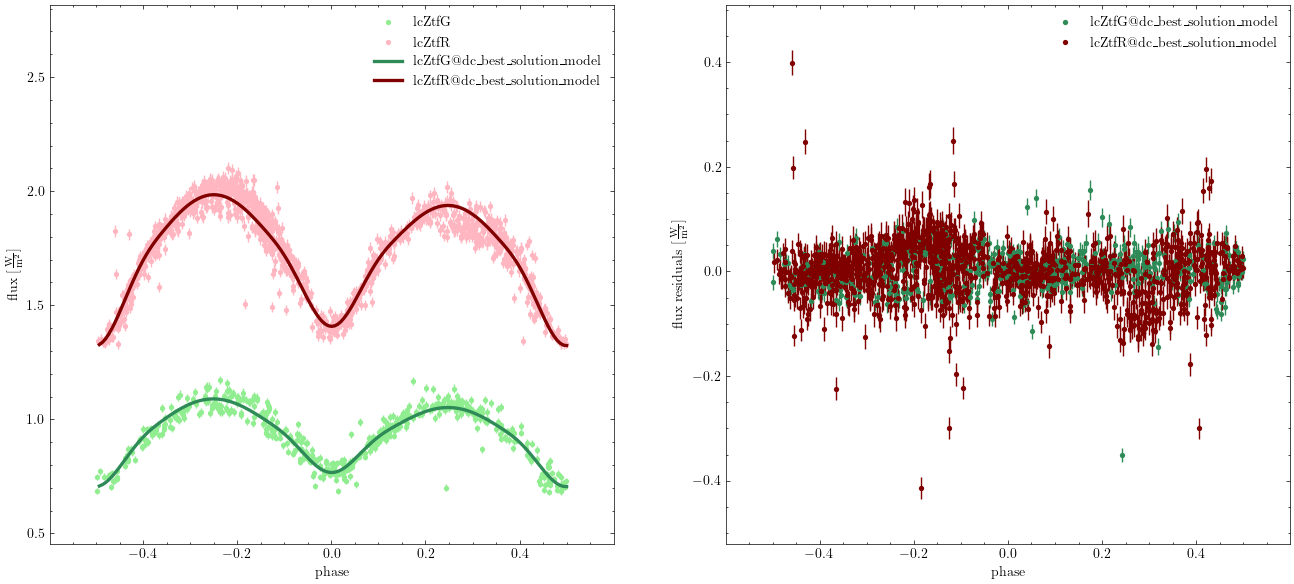
\includegraphics[scale=0.5]{Metodologia/Secciones/ModeloComputacional/Figures/Figura Opt DC Resultados ZTF.png}
	\caption{Modelo sintético junto a el residuo de flujo tomando en cuenta una
	mancha estelar fría en la componente secundaria (vista en la
	\reffigure{figuraMallaManchaNm}) y utilizando los parámetros resultados del
	proceso de optimización vistos en la \reftable{tablaOptDcResultados}.}
	\label{figuraOptDcResultadosZtf}
\end{figure}

\section{Ajuste de Luminosidad y Temperatura Efectiva}

Utilizando las curvas calibradas de ZTF en ambas pasabandas se determinó la
temperatura efectiva del sistema partiendo unicamente de las curvas
fotométricas. Para esto se manipularon en total 3 parámetros del sistema: la
temperatura efectiva de la componente primaria (\code{teff@primary}), la razón
de temperaturas de las componentes $T_2 / T_1$ (\code{teffratio}), y el factor
de escala de la luminosidad de pasabanda (\code{pblum@primary@lcZtfG}) para la
pasabanda ZTF:g. Se acopló la temperatura efectiva del sistema al color (dado
por el flujo relativo entre las curvas de ZTF) utilizando el modo
\code{pblum\_mode} con el valor \code{component-coupled} para la curva de ZTF:g,
y un valor de \code{dataset-coupled} para la curva de ZTF:r. En el modo
\code{component-coupled} el usuario proporciona un valor para la luminosidad
emergente de la componente primaria en el tiempo $t_0$ del sistema, a partir del
cual PHOEBE determina un factor de escala tal que las intensidades superficiales
de las estrellas sean igual a la luminosidad dada. El modo
\code{dataset-coupled} aplica el mismo factor de escala a la curva de ZTF:r que
el factor dado a la curva ZTF:g, manteniendo información del color del sistema
[\citeyearparen{conroy_phoebe_v_framework_solving_inverse_problem_2020}]. 

Una vez que se haya establecido esta configuración del bundle se aplicó un
optimizador de tipo NMS para ajustar los tres parámetros mencionados en el
párrafo pasado. Como valor inicial se ajustó manualmente la temperatura efectiva
de la primaria a $4600 \ \mathrm{K}$, el cual se determinó por medio de
experimentación manual. Después de 174 iteraciones el optimizador logró
converger a la solución dada en la \reftable{tablaOptNmTeffResultados}. Dado que
estos parámetros principalmente afectan el factor de escala de las curvas de
luz, los demás parámetros del sistema se mantuvieron fijos, manteniendo la forma
de las curvas de luz.

% TODO: style table
\begin{table}[!ht]
	\centering
	\begin{tabular}{|l|l|}
		\hline
		% \rowcolor{blue}
		\thead{Parámetro}                        & \thead{Valor optimizado} \\
		\hline
		\code{teff@primary}							& 4203.69115 K  \\
		\hline
		\code{teffratio@binary}						& 1.05213       \\
		\hline
		\code{pblum@primary@lcZtfG}					& 4.78643 W       \\
		\hline
	\end{tabular}
	\caption{Valores optimizados para la temperatura efectiva de la estrella
	primaria, junto a la luminosidad de pasabanda que produce el factor de
	escala necesario para ajustar a la curva fotométrica. La temperatura
	efectiva de la secundaria está constreñida por la temperatura efectiva de la
	primaria y la razón de temperaturas; dado estos parámetros, la temperatura
	efectiva secundaria es igual a 4422.837561158592 K.}
	\label{tablaOptNmTeffResultados}
\end{table}

\section{Muestreo MCMC}

Una vez que se haya obtenido el conjunto de parámetros que mejor ajustan el
modelo sintético a los datos observacionales se busca obtener las incertidumbres
para cada parámetro. La manera recomendada por el equipo de desarrollo de PHOEBE
es por medio de un muestreo Bayesiano \textit{Monte Carlo Markov Chain}.
Utilizando un muestreo MCMC es posible determinar la morfología del espacio de
parámetros de manera holística; esto permite identificar cualquier correlación
que exista entre los parámetros del sistema. El proceso de muestreo empleado en
este proyecto es por PHOEBE utilizando el paquete de Python \code{emcee},
descrito en la \refthesissubsection{intro:phoebe:problema_inverso:muestreo}.
Antes de correr el proceso de muestreo se preparó el bundle de la siguiente
manera.

\subsection{Eliminación de Observaciones Erróneas}

PHOEBE utiliza la probabilidad logarítmica ($\mathrm{lnprobability}$) del modelo
sintético como la \textit{función de merito} para el muestreo. Esta se define en
la siguiente ecuación:

\begin{eqfloat}[!ht]
	\centering
	\begin{equation}
		\textrm{lnprobability} = \textrm{lnpriors} + \textrm{lnlikelihood}
	\end{equation}
\end{eqfloat}

Donde $\mathrm{lnpriors} = \sum_{\Pi} \ln{P(p | \pi)}$ es la probabilidad
logarítmica de obtener los parámetros actuales del modelo $p$ de una
distribución a priori $\pi$ sumando sobre todas las distribuciones priores $\Pi$
[\citeyearparen{conroy_phoebe_v_framework_solving_inverse_problem_2020}]. El
término $\mathrm{lnlikelihood}$ es la verosimilitud, la cual está definido por
la \refequation{ecuacionLnLikelihoodMcmc}. Tras varios experimentos corriendo
varias instancias del muestreo MCMC se descubrió que los caminadores son
excepcionalmente sensibles a fluctuaciones en la función de merito; las
observaciones que se desvían de manera significativa de la región principal de
la curva de luz en fase indican un ajuste inadecuado según la función de merito.
Debido a que las incertidumbres de estos puntos probablemente fueron registrados
de manera errónea se eliminaron estos puntos de la curva observada. En el
Notebook
\href{https://github.com/KnightIV/UANL_MAPTA_Observaciones/blob/main/analisis/phoebe_model/sampling/remove-bad-observations.ipynb}{\code{remove-bad-observations.ipynb}}
se aplicó un criterio al desviación estándar de los residuos del modelo
optimizado; aquellos puntos cuya diferencia con el modelo sintético sea mayor de
un múltiple de la desviación estándar fue eliminado de los datos. Los resultados
de esta optimización se pueden ver en la
\reffigure{figuraEliminarMalasObservacionesZtf}. El modelo sintético utilizando
solo estos datos se puede ver en la
\reffigure{figuraModeloSinMalasObservacionesZtf}, donde se puede apreciar a
mayor detalle la forma oscilatoria de los residuos. Esto indica que los valores
obtenidos no son los óptimos y aún hay más cambios que se podrían emplear para
llegar a un mejor ajuste; sin embargo, este es un ajuste suficientemente bueno
para este proyecto para continuar al muestreo del espacio de parámetros con
MCMC.

\begin{figure}[!ht]
	\centering
	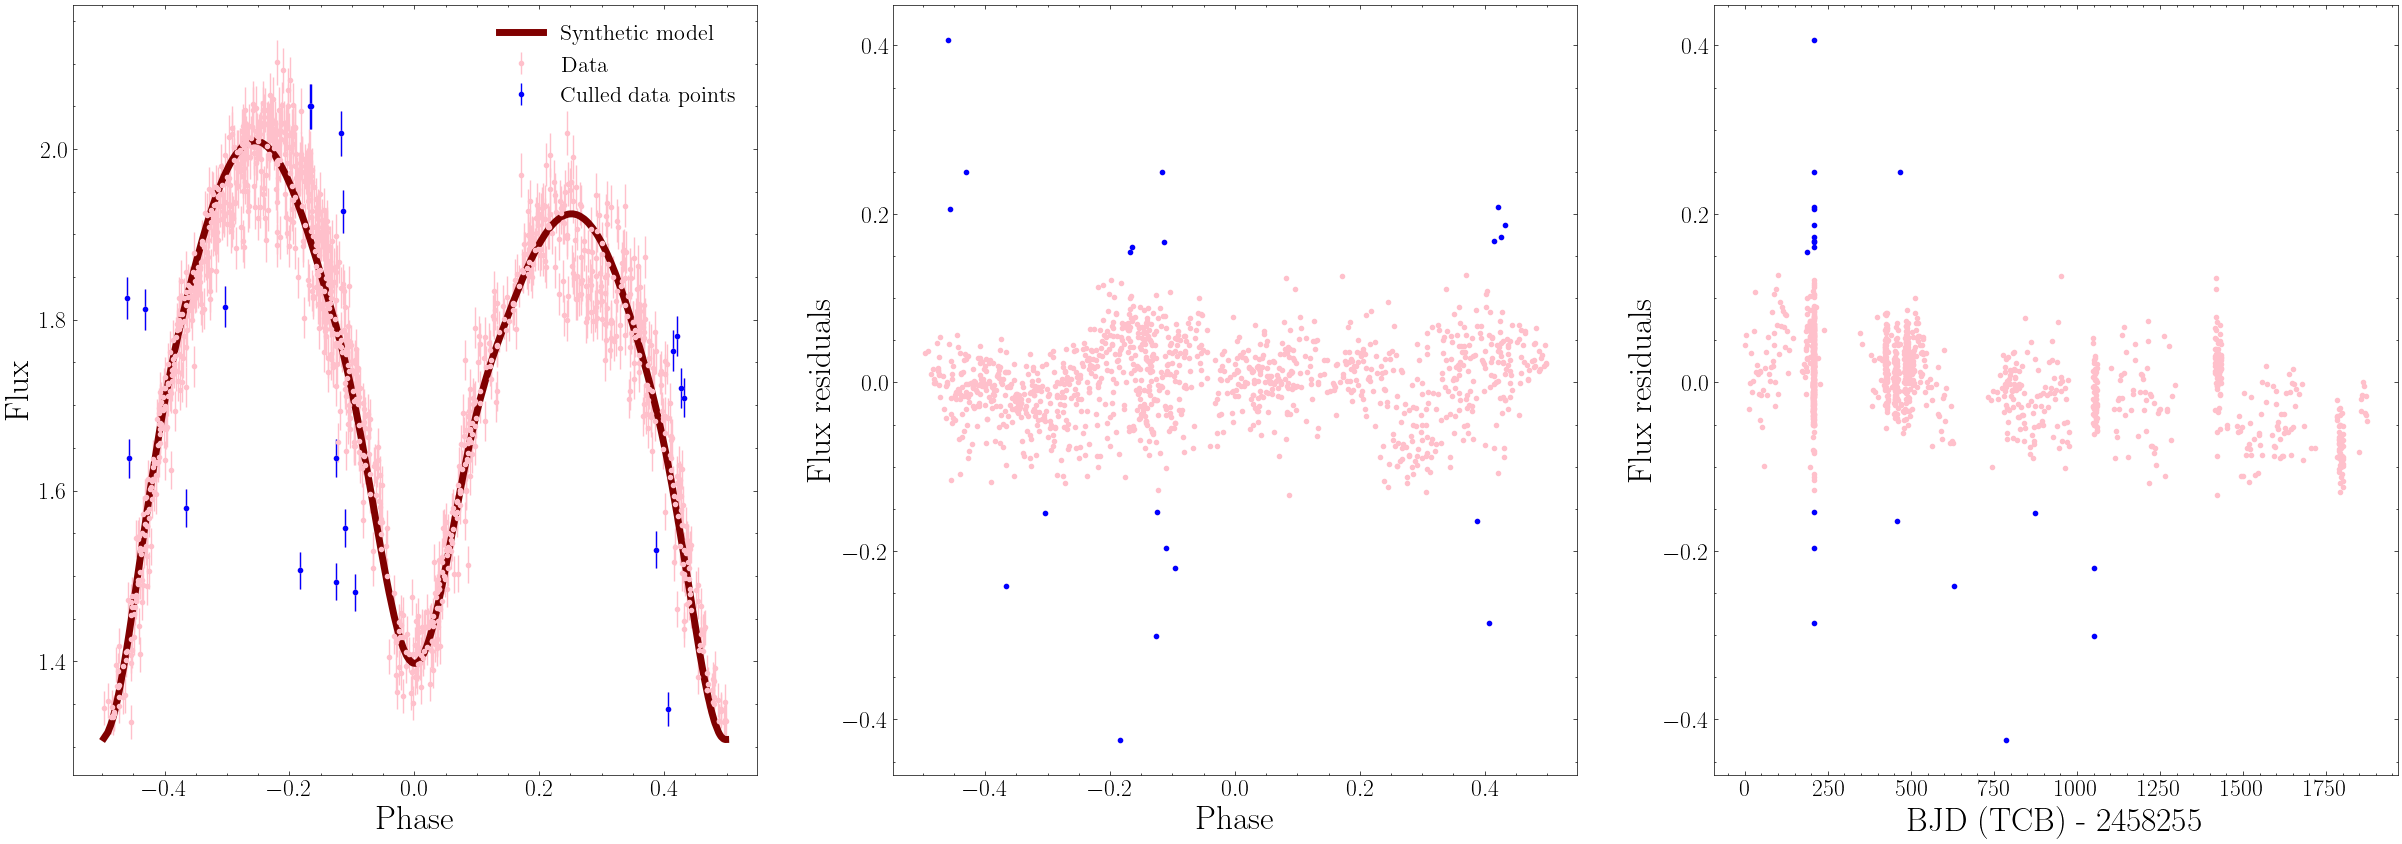
\includegraphics[scale=0.27]{Metodologia/Secciones/ModeloComputacional/Figures/Figura Malas Observaciones ZTF:r.png}
	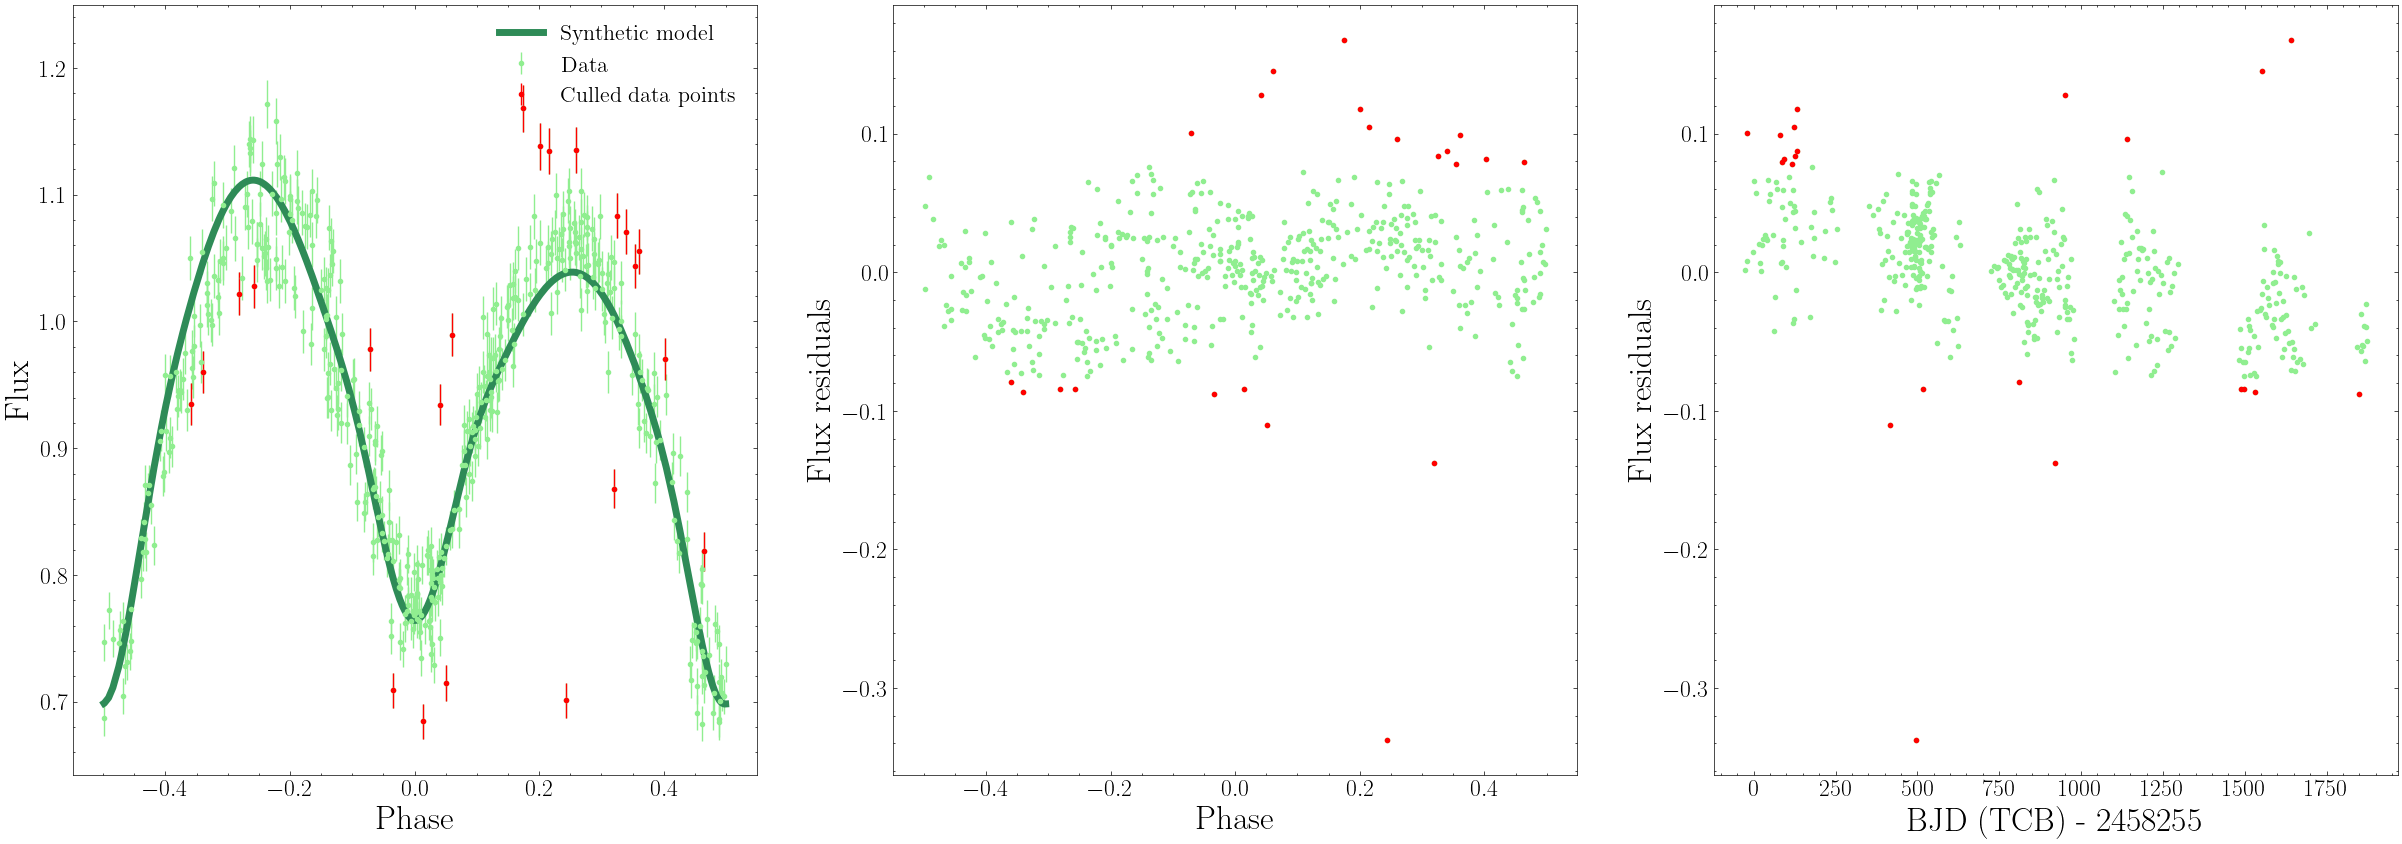
\includegraphics[scale=0.27]{Metodologia/Secciones/ModeloComputacional/Figures/Figura Malas Observaciones ZTF:g.png}
	\caption{Resultados de aplicar el criterio de eliminación para las curvas de
	luz de ZTF, donde la figura superior corresponde a la pasabanda ZTF:r y la
	inferior a ZTF:g. Se optó por codificar este criterio en el código en vez de
	eliminar los datos manualmente para ser fácilmente reproducible. El factor
	de escala del criterio fue ajustado manualmente tal que los puntos más
	erróneos sean eliminados con éxito, y al mismo tiempo preservar la forma y
	dispersión principal que existen en los datos.}
	\label{figuraEliminarMalasObservacionesZtf}
\end{figure}

\begin{figure}[!ht]
	\centering
	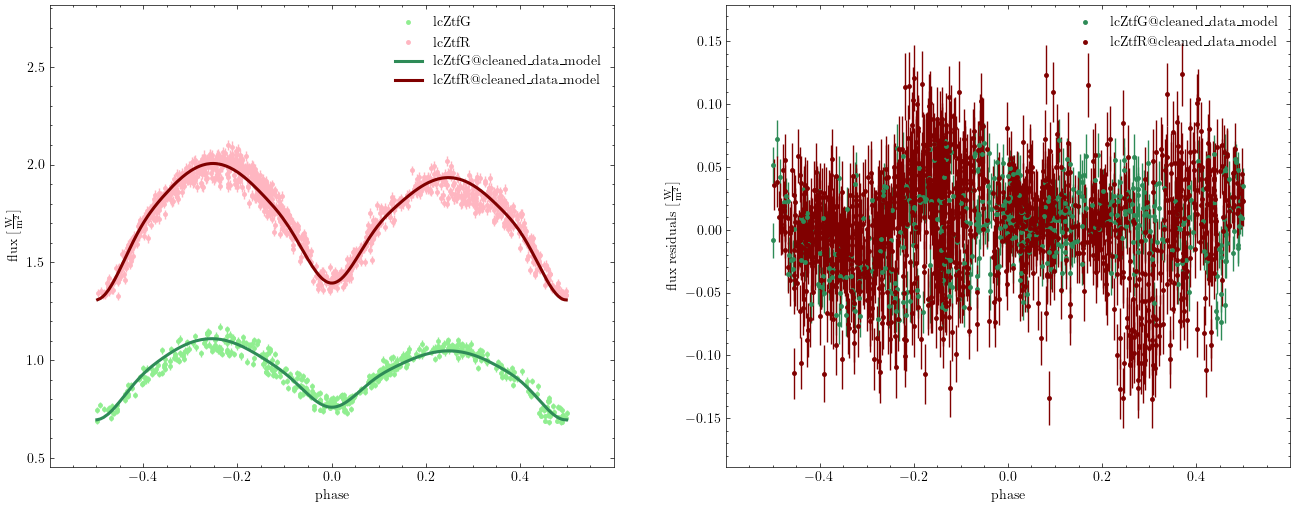
\includegraphics[scale=0.5]{Metodologia/Secciones/ModeloComputacional/Figures/Figura Modelo Sin Malas Observaciones ZTF.png}
	\caption{Modelo sintético en las pasabandas de ZTF calculado después de
	eliminar las observaciones más problemáticas de las curvas observadas.}
	\label{figuraModeloSinMalasObservacionesZtf}
\end{figure}

\subsection{Distribuciones Priores}

Para poder muestrear el espacio de parámetros, el algoritmo MCMC requiere de una
región inicial a partir de cual inicializar las posiciones de cada caminador.
Estas distribuciones iniciales también actúa como una guía; al principio del
muestreo los caminadores en su mayoría no saldrán de las regiones de
concentración de estas distribuciones. La forma de las priores dejará de
importar tanto entre más iteraciones logre correr la cadena, de la cual se
estimará la distribución posterior de densidad de cada parámetro.

PHOEBE ofrece unas herramientas para los tipos de distribuciones más comunes en
este trabajo: la distribución uniforme y la distribución Gaussiana (normal).
Para el muestreo de \atoObjId se utilizaron distribuciones uniformes para los
parámetros ajustables del bundle\textemdash todos aquellos que han sido
ajustados a lo largo de la optimización de parámetros. Una distribución uniforme
no tiene un significado físico intrínseco más allá de comunicar una falta de
información del problema. En nuestro caso, las priores sirven para marcar un
límite práctico para cada parámetro, tanto para evitar que los caminadores se
pierdan en espacios que produzcan un resultado no físico, cómo para constreñir
el volumen de interés a lo más cercano de los parámetros óptimos derivados en el
proceso de optimización. 

Se crearon 3 colecciones de distribuciones en el bundle de PHOEBE para delimitar
los parámetros ajustables del modelo: 1 para los parámetros de interés del
sistema binario, 1 para los parámetros que rigen la mancha estelar en la
componente secundaria, y 1 que restringe el factor de escala en la pasabanda
ZTF:g. Las colecciones individuales de distribuciones priores se pueden ver en
la \reffigure{figuraColeccionesPrioresZtf}, la
\refthesissection{apendice:modelo_computacional_graficas:dist_priores_completas}
muestra todos los priores utilizados para el proceso de MCMC.

\begin{figure}[!ht]
	\centering
	\xincludegraphics[scale=0.29, label=\textbf{a)}, labelbox=true, pos=ne, fontsize=\Large]{Metodologia/Secciones/ModeloComputacional/Figures/Figura Prior Params Binaria.png}
	\xincludegraphics[scale=0.345, label=\textbf{b)}, labelbox=true, pos=ne, fontsize=\Large]{Metodologia/Secciones/ModeloComputacional/Figures/Figura Prior Params Mancha.png}
	\xincludegraphics[scale=0.85, label=\textbf{c)}, labelbox=true, pos=ne, fontsize=\Large]{Metodologia/Secciones/ModeloComputacional/Figures/Figura Prior Params Luminosidad ZTF.png}
	\caption{Distribuciones priores utilizadas como límites iniciales a cada
	caminador. Se separaron en 3 distintas colecciones por cuestiones de
	organización dentro del código: \textbf{a)} los parámetros principales del
	sistema solar que afectan la forma de la curva fotométrica sintética en
	orden de izquierda a derecha y de arriba a abajo: la temperatura efectiva de
	la componente primaria ($T_{1}$), la razón de temperaturas ($T_2/T_1$), el
	factor de relleno ($f$), la inclinación orbital ($i_{\mathrm{orb}}$), y la
	razón de masas ($q$). \textbf{b)} los parámetros de la mancha estelar en la
	componente secundaria que se introdujo para tomar en cuenta el efecto
	O'Connell: su posición con respecto al origen del sistema de coordenadas en
	la secundaria (la longitud y latitud de la mancha), el radio angular, y la
	razón de temperatura de la mancha con respecto a la temperatura efectiva
	local de la superficie de la componente secundaria. \textbf{c)} la
	luminosidad en la pasabanda ZTF:g, la cual determina el factor de escala de
	las curvas de luz; este parámetro fue incluido en el muestreo para permitir
	integrar sobre este \textit{parámetro molesto}, ya que tiene un efecto
	significativo en la curva sintética pero no es un parámetro que nos interese
	medir directamente.}
	\label{figuraColeccionesPrioresZtf}
\end{figure}

\section{Distribuciones de Probabilidad Posterior}

